\chapter{Tính toán trục}
\section{Chọn vật liệu và tính sơ bộ}
Vì chưa biết chiều dài trục nên ta thiết kế sơ bộ để xác định đường kính trục theo moment xoắn. 
Chọn vật liệu chế tạo trục là thép C45 tôi cải thiện. Do trục bánh răng trong hộp giảm tốc là chi tiết máy rất quan trọng.

Tra bảng thông số vật liệu ta có thông số cơ tính của vật liệu như sau:
\begin{itemize}
    \item Loại thép: 45
    \item Nhiệt luyện: tôi cải thiện
    \item Độ rắn: $HB_1 = 260 \, \text{HB}$
    \item Giới hạn bền: $\sigma_b = 850 \, \text{MPa}$
    \item Giới hạn chảy: $\sigma_{ch} = 650 \, \text{MPa}$
\end{itemize}
Chọn ứng suất xoắn cho phép $[\tau] = 20 \, \text{MPa}$ \\
Xác định sơ bộ đường kính trục:
\[
d_1 \geq \sqrt[3]{\frac{T_1}{0.2[\tau]}} = \sqrt[3]{\frac{65914.47}{0.2 \cdot 20}} = 25.44 \text{mm}
\]
\[
d_2 \geq \sqrt[3]{\frac{T_2}{0.2[\tau]}} = \sqrt[3]{\frac{321365.99}{0.2 \cdot 20}} = 37.69 \text{mm}
\]
Tra bảng 10.2 tài liệu [2], ta chọn sơ bộ đường kính trục và bề rộng ổ lăn theo tiêu chuẩn:
\begin{itemize}
    \item Trục I: $d_1 = 25.44 \, \text{mm}$; $b_{o1} = 19 \, \text{mm}$
    \item Trục II: $d_2 = 35 \, \text{mm}$; $b_{o2} = 25 \, \text{mm}$  
\end{itemize}
\section{Xác định khoảng cách giữa các ổ lăn và điểm đặt lực}
\subsection{Trục I}
Theo bảng 10.3 tài liệu [2], ta có:
\begin{itemize}
    \item $k_1 = 8$ mm: Khoảng cách từ mặt mút của chi tiết quay đến thành trong của hộp hoặc khoảng cách giữa các chi tiết quay
    \item $k_2 = 10$ mm: Khoảng cách từ mặt mút ổ đến thành trong của hộp
    \item $k_3 = 10$ mm: Khoảng cách từ mặt mút của chi tiết quay đến nắp ổ
    \item $h_n = 15$ mm: Chiều cao nắp ổ và đầu bu lông
    \item Chọn sơ bộ chiều dài mayơ bánh răng trụ dẫn: $l_{m13}$ = bề dày bánh răng $b_w$ = 70 mm
    \item Chọn sơ bộ chiều dài mayơ bánh đai: $l_{m12} = (1.2\div 1.5)d_1 = 30 \div 37.5$. Chọn $l_{m22}=36$ mm 
    \item $l_{13} = 0.5(l_{m13} + b_{o1}) + k_1 + k_2 = 0.5(70 + 21) + 10 + 8 = 63.5 \, \text{mm}$
    \item $l_{11} = 2l_{13} = 2 \cdot 63.5 = 127 \, \text{mm}$
 
    \item $l_{12} = 0.5(l_{m12} + b_{o1}) + k_3 + h_n = 0.5(50 + 21) + 10 + 15 = 75.5 \, \text{mm}$
\end{itemize}

\subsection{Trục II}
Theo bảng 10.3 tài liệu [2], ta có:
\begin{itemize}
    \item $k_1 = 8$ mm: Khoảng cách từ mặt mút của chi tiết quay đến thành trong của hộp hoặc khoảng cách giữa các chi tiết quay
    \item $k_2 = 10$ mm: Khoảng cách từ mặt mút ổ đến thành trong của hộp
    \item $k_3 = 10$ mm: Khoảng cách từ mặt mút của chi tiết quay đến nắp ổ
    \item $h_n = 15$ mm: Chiều cao nắp ổ và đầu bu lông
    \item $l_{m23}$ = bề dày bánh răng $b_w$ = 64 mm
    \item $l_{m22} = (1.2\div 1.5)d_1 = 45.25 \div 57$. Chọn $l_{m22}=57$ mm
    \item $l_{23} = 0.5(l_{m13} + b_{o1}) + k_1 + k_2 = 64.5 \, \text{mm}$
    \item $l_{21} = 0.5(l_{m23} + b_{o2}) + k_1 + k_2 = 140.5 \, \text{mm}$
    \item $l_{22} = 2l_{21}$ = 
\end{itemize}

\section{Phân tích lực tác dụng}
\subsection{Trục I}
\begin{itemize}
    \item Lực vòng: $F_{t1}$ = 2471.8 N
    \item Lực dọc trục: $F_{a1}$ = 756.18 N
    \item Lực hướng tâm: $F_{r1}$ = 940.82 N 
    \item Lực do bộ truyền đai: $F_d$ = 474.74 N
\end{itemize}
\subsection{Trục II}
\begin{itemize}
    \item Lực vòng: $F_{t2}$ = 2471.8 N
    \item Lực dọc trục: $F_{a2}$ = 940.82 N
    \item Lực hướng tâm: $F_{r2}$ = 756.18 N 
    \item Lực nối trục: $F_{nt}$ = 1483.23 N
\end{itemize}
\section{Tính momen tương đương và đường kính trục}
\subsubsection{Trục I}
Moment do lực dọc trục tạo ra:
\[
    M_{a1} = F_{a1} \cdot \frac{d_1}{2} 
           = 756.177 \cdot \frac{53.33}{2} 
           = 20163.47\ \text{Nmm}
\]
\[
    \left\{
    \begin{array}{l}
        \sum F_X = 0 \\
        \sum F_Y = 0 \\
        \sum M_{Y/A} = 0 \\
        \sum M_{X/A} = 0
    \end{array}
    \right.
    \Leftrightarrow
    \left\{
    \begin{array}{l}
        -F_{dy} - R_{BY} + F_{r1} - R_{DY} = 0 \\
        -F_{dy} - R_{BY} + F_{r1} - R_{DY} = 0  \\
        -63{,}5 F_{t1} + 127 R_{BX} = 0 \\
        75{,}5 F_{r1}^d + 63{,}5 F_{r1} - M_{a1} - 127 R_{BY} = 0
    \end{array}
    \right.
    \Leftrightarrow
    \left\{
    \begin{array}{l}
        R_{AX} = 1390{,}89\ \text{N} \\
        R_{AY} = 2236{,}88\ \text{N} \\
        R_{BX} = 1984{,}15\ \text{N} \\
        R_{BY} = 899{,}7\ \text{N}
    \end{array}
    \right.
\]

Theo bảng 10.5 tài liệu [1], với $d_1 = 35\ \text{mm} \rightarrow [\sigma] = 63\ \text{MPa}$

\[
    M_E^{td} 
    = \sqrt{M_{X/E}^2 + M_{Y/E}^2 + 0.75 \cdot T_E^2} 
    = \sqrt{0.75 \cdot 144308.115^2} 
    = 124975\ \text{Nmm}
\]

\[
    M_A^{td} 
    = \sqrt{M_{X/A}^2 + M_{Y/A}^2 + 0.75 \cdot T_A^2} 
    = \sqrt{59645^2 + 0.75 \cdot 144308.115^2} 
    = 138478\ \text{Nmm}
\]

\[
    M_F^{td} 
    = \sqrt{M_{X/F}^2 + M_{Y/F}^2 + 0.75 \cdot T_F^2} 
    = \sqrt{62159.1^2 + 125993.5^2 + 0.75 \cdot 144308.115^2}
    \Rightarrow M_F^{td} = 188034\ \text{Nmm}
\]

\[
    M_B^{td} 
    = \sqrt{M_{X/B}^2 + M_{Y/B}^2 + 0.75 \cdot T_B^2} 
    = 0\ \text{Nmm}
\]

\[
    d_A \ge \sqrt[3]{\frac{M_A^{td}}{0.1 \cdot \sigma}} 
        = \sqrt[3]{\frac{138478}{0.1 \cdot 63}} 
        = \sqrt[3]{\frac{138478}{6.3}} 
        = \sqrt[3]{21979.68} 
        = 28.01\ \text{mm}
\]

\[
    d_E \ge 27.07\ \text{mm}; \quad d_F \ge 31.02\ \text{mm}
\]

Theo kết cấu và tiêu chuẩn ta chọn:
\[
    d_A = d_B = 30\ \text{mm}; \quad d_E = 28\ \text{mm}; \quad d_F = 35\ \text{mm}
\]
\begin{figure}[H]
    \centering
    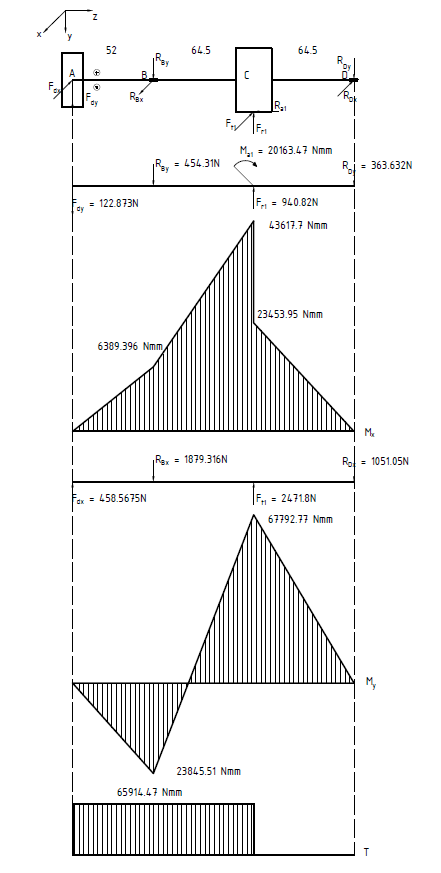
\includegraphics[width=0.7\textwidth]{pictures/momen1.png}
\end{figure}

\subsection{Trục II}
Moment do lực dọc trục tạo ra:
\[
    M_{a1} = F_{a1} \cdot \frac{d_1}{2} 
           = 1118{,}4 \cdot \frac{72{,}73}{2} 
           = 40670{,}6\ \text{Nmm}
\]
\[
    \left\{
    \begin{array}{l}
        \sum F_X = 0 \\
        \sum F_Y = 0 \\
        \sum M_{Y/A} = 0 \\
        \sum M_{X/A} = 0
    \end{array}
    \right.
    \Leftrightarrow
    \left\{
    \begin{array}{l}
        -R_{AX} - R_{BX} + F_{t1} = 0 \\
        -F_{r1}^d + R_{AY} - F_{r1} + R_{BY} = 0 \\
        -63{,}5 F_{t1} + 127 R_{BX} = 0 \\
        75{,}5 F_{r1}^d + 63{,}5 F_{r1} - M_{a1} - 127 R_{BY} = 0
    \end{array}
    \right.
    \Leftrightarrow
    \left\{
    \begin{array}{l}
        R_{AX} = 1390{,}89\ \text{N} \\
        R_{AY} = 2236{,}88\ \text{N} \\
        R_{BX} = 1984{,}15\ \text{N} \\
        R_{BY} = 899{,}7\ \text{N}
    \end{array}
    \right.
\]

Theo bảng 10.5 tài liệu [1], với $d_1 = 35\ \text{mm} \rightarrow [\sigma] = 63\ \text{MPa}$

\[
    M_E^{td} 
    = \sqrt{M_{X/E}^2 + M_{Y/E}^2 + 0.75 \cdot T_E^2} 
    = \sqrt{0.75 \cdot 144308.115^2} 
    = 124975\ \text{Nmm}
\]

\[
    M_A^{td} 
    = \sqrt{M_{X/A}^2 + M_{Y/A}^2 + 0.75 \cdot T_A^2} 
    = \sqrt{59645^2 + 0.75 \cdot 144308.115^2} 
    = 138478\ \text{Nmm}
\]

\[
    M_F^{td} 
    = \sqrt{M_{X/F}^2 + M_{Y/F}^2 + 0.75 \cdot T_F^2} 
    = \sqrt{62159.1^2 + 125993.5^2 + 0.75 \cdot 144308.115^2}
    \Rightarrow M_F^{td} = 188034\ \text{Nmm}
\]

\[
    M_B^{td} 
    = \sqrt{M_{X/B}^2 + M_{Y/B}^2 + 0.75 \cdot T_B^2} 
    = 0\ \text{Nmm}
\]

\[
    d_A \ge \sqrt[3]{\frac{M_A^{td}}{0.1 \cdot \sigma}} 
        = \sqrt[3]{\frac{138478}{0.1 \cdot 63}} 
        = \sqrt[3]{\frac{138478}{6.3}} 
        = \sqrt[3]{21979.68} 
        = 28.01\ \text{mm}
\]

\[
    d_E \ge 27.07\ \text{mm}; \quad d_F \ge 31.02\ \text{mm}
\]

Theo kết cấu và tiêu chuẩn ta chọn:
\[
    d_A = d_B = 30\ \text{mm}; \quad d_E = 28\ \text{mm}; \quad d_F = 35\ \text{mm}
\]
\begin{figure}[H]
    \centering
    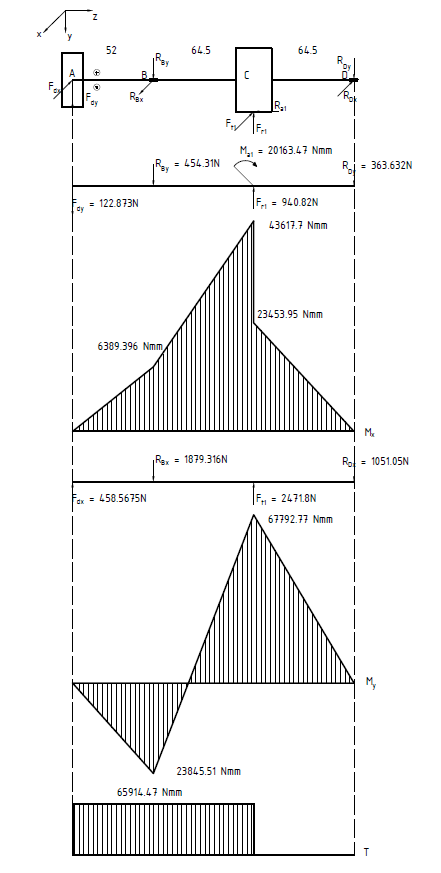
\includegraphics[width=0.7\textwidth]{pictures/momen1.png}
\end{figure}

\section{Chọn và kiểm nghiệm then}
\begin{itemize}
    \item Dựa vào bảng 9.1 là tài liệu [2], chọn kích thước then BXH theo tiết diện lớn nhất của trước.
    \item Chọn chiều dài $l$, theo tiêu chuẩn của then, nhỏ hơn chiều dài mayơ $l_m = 5 \div 10$ mm.
    \item Kiểm nghiệm then theo độ bền đập và độ bền cắt then băng
    \[
    \sigma_d = \frac{2T}{d l_w (h - t_1)} \leq [\sigma_d] \quad \tau_c = \frac{2T}{d l_w b} \leq [\tau_c]
    \]
    Với
    \[
    [\sigma_d] = 150 \, \text{MPa}, \text{tra theo bảng 9.5 tài liệu \cite{2}}
    \]
    \[
    [\tau_c] = 60 \div 90 \, \text{MPa}
    \]
    $l_w = l - b$: chiều dài làm việc của then băng 2 đầu tròn
\end{itemize}
\textbf{Bảng thông số:}
\begin{center}
\begin{tabular}{|l|c|c|c|c|c|c|c|c|c|c|c|}
\hline
\textbf{Trục} & \textbf{Đường kính} & \textbf{Mặt cắt} & $l_m$ & $l$ & $l_w$ & $b$ & $h$ & $t_1$ & $\sigma_d$ & $\tau_c$ & $T$ \\
\hline
\multirow{2}{*}{\textbf{I}} & 28 & 12 & 45 & 40 & 32 & 8 & 7 & 4 & 107,4 & 40,3 & 1443308,115 \\
\cline{2-12}
& 35 & 13 & 70 & 65 & 55 & 10 & 8 & 5 & 49,97 & 15,0 & 1443308,115 \\
\hline
\multirow{2}{*}\textbf{II} & 55 & 22 & 75 & 70 & 54 & 16 & 10 & 6 & 101,1 & 25,3 & 600394,168 \\
\cline{2-12}
& 46 & 23 & 75 & 70 & 56 & 14 & 9 & 5,5 & 127,6 & 31,9 & 600394,168 \\
\hline
\end{tabular}
\end{center}

$\Rightarrow$ Các mặt cắt đều thỏa điều kiện bền đập và căng bền đảm bảo an toàn cho phép.

\section{Kiểm nghiệm độ bền trục}
\subsection{Độ bền mỏi}
Hệ số an toàn:
\[
s = \frac{s_0 s_\tau}{\sqrt{s_0^2 + s_\tau^2}} \geq [s]
\]
\begin{itemize}
    \item Với hệ số an toàn cho phép $[s] = 1.5 \div 2.5$, khi tăng độ căng $[s] = 2.5 \div 3$, nhưng vậy không cần kiểm nghiệm về độ căng.
    \item $s_0, s_\tau$ hệ số an toàn chi xét riêng ứng suất pháp, ứng suất tiếp
    \[
    s_0 = \frac{K_0 \sigma_a + \psi_0 \sigma_m}{\varepsilon_\beta \sigma}, \quad s_\tau = \frac{K_\tau \tau_a + \psi_\tau \tau_m}{\varepsilon_\tau \tau}
    \]
    \item $\sigma_{-1}, \tau_{-1}$ giới hạn mỏi của vật liệu tính theo công thức:
    \[
    \sigma_{-1} = (0.4 \div 0.5) \sigma_b = 240 \div 300 \, \text{MPa}, \text{ chọn } \sigma_{-1} = 280 \, \text{MPa}
    \]
    \[
    \tau_{-1} = (0.22 \div 0.25) \sigma_b = 132 \div 150 \, \text{MPa}, \text{ chọn } \tau_{-1} = 140 \, \text{MPa}
    \]
    \[
    \sigma_b = 600 \, \text{MPa}: \text{giới hạn bền của thép 45 thường hóa}
    \]
    Theo bảng 10.8 tài liệu [1], $K_0 = 1.75$, $K_\tau = 1.5$
    \item $\sigma_a, \sigma_m, \tau_a, \tau_m$: biên độ và giá trị của ứng suất. Vì tất cả các trục của hợp giảm tốc đều quay nên ứng suất thay đổi theo chu kỳ đối xứng: $\sigma_m = 0$, $\sigma_a = \sigma_{\text{max}} = \frac{M}{W}$, với $M$ là moment uốn thương trường, $W$ là moment chóng uốn
    \item Đo trực quy 1 chiều nên ứng suất xoắn thay đổi theo chu kỳ mạch động
\end{itemize}
\[
\tau_a = \tau_m = \frac{T_{\text{max}}}{2}, \quad \text{với } W_0 \text{ là moment chống xoắn, } T \text{ là moment xoắn}
\]
\begin{itemize}
    \item $\psi_\sigma = 0.05; \psi_\tau = 0$ hệ số xét đến ảnh hưởng của ứng suất trung bình đến độ bền mỏi của vật liệu
    \item $\varepsilon_\sigma, \varepsilon_\tau$: hệ số kích thước (bảng 10.3 tài liệu [1])
    \item $\beta = 1.7$: hệ số tăng bề mặt (bảng 10.5 tài liệu [1])
\end{itemize}
\subsection{Độ bền tĩnh}
Để đề phòng trục bị biến dạng dẻo quá lớn hoặc bị gãy khi bị quá tải đột ngột ta cần kiểm nghiệm trục theo độ bền tĩnh:

\begin{itemize}
    \item Công thức thực nghiệm cơ dạng: $\sigma_d = \sqrt{\sigma^2 + 3\tau^2} \leq [\sigma_d]_t$
\end{itemize}

Trong đó:
\[
\sigma = \frac{M}{W} = \sigma_a; \quad \tau = \frac{T}{W_0} = 2\tau_a; \quad [\sigma_d]_t \approx 0.8\sigma_{ch} = 0.8340 = 272 \, \text{MPa}
\]

\textbf{Bảng kết quả tính toán}

\begin{center}
\begin{tabular}{|l|c|c|c|c|c|c|c|c|c|c|c|}
\hline
\textbf{Trục} & \textbf{Tiết diện} & $W$ & $W_0$ & $\sigma_a$ & $\tau_a$ & $\sigma_d$ & $\varepsilon_\sigma$ & $\varepsilon_\tau$ & $s_\sigma$ & $s_\tau$ & $s$ \\
\hline
\multirow{3}{*}{\textbf{I}} & 10 & 2128.5 & 4777.9 & 21.5 & 15.1 & 33.9 & 0.88 & 0.81 & 11.13 & 8.51 & 6.76 \\
\cline{2-12}
& 12 & 1824.9 & 3978.9 & 0 & 18.1 & 31.4 & 0.91 & 0.89 & -- & 7.8 & -- \\
\cline{2-12}
& 13 & 3564.3 & 7771.4 & 37.5 & 9.3 & 40.8 & 0.88 & 0.81 & 6.38 & 13.8 & 5.79 \\
\hline
\multirow{3}{*}{\textbf{II}} & 21 & 10407.1 & 22672.7 & 11.1 & 13.2 & 25.5 & 0.81 & 0.76 & 19.85 & 9.14 & 8.3 \\
\cline{2-12}
& 22 & 14230.1 & 30555.7 & 17.2 & 9.8 & 24.2 & 0.81 & 0.76 & 12.81 & 12.3 & 8.87 \\
\cline{2-12}
& 23 & 9403.1 & 20254.9 & 0 & 14.82 & 25.7 & 0.84 & 0.78 & -- & 8.35 & -- \\
\hline
\end{tabular}
\end{center}

Vậy các trục thỏa điều kiện bền mỏi và độ bền tĩnh